\documentclass[a5paper]{article}
\usepackage[a5paper, top=8mm, bottom=8mm, left=8mm, right=8mm]{geometry}

\usepackage{polyglossia}
\setdefaultlanguage[babelshorthands=true]{russian}

\usepackage{fontspec}
\setmainfont{FreeSerif}
\newfontfamily{\russianfonttt}[Scale=0.7]{DejaVuSansMono}

\usepackage[font=scriptsize]{caption}

\usepackage{amsmath}
\usepackage{amssymb,amsfonts,textcomp}
\usepackage{color}
\usepackage{array}
\usepackage{hhline}
\usepackage{cite}

\usepackage[hang,multiple]{footmisc}
\renewcommand{\footnotelayout}{\raggedright}

\PassOptionsToPackage{hyphens}{url}\usepackage[xetex,linktocpage=true,plainpages=false,pdfpagelabels=false]{hyperref}
\hypersetup{colorlinks=true, linkcolor=blue, citecolor=blue, filecolor=blue, urlcolor=blue, pdftitle=1, pdfauthor=, pdfsubject=, pdfkeywords=}

\usepackage{tabu}

\usepackage{graphicx}
\usepackage{indentfirst}
\usepackage{multirow}
\usepackage{subfig}
\usepackage{footnote}
\usepackage{minted}

\sloppy
\pagestyle{plain}

\title{Лекция 2: Введение в F\#}

\date{}

\begin{document}

\maketitle
\thispagestyle{empty}

\section{Введение}

F\# --- это типизированный функциональный язык для платформы .NET, появившийся в 2005 году как альтернатива C\#. Язык, в отличие от Haskell, не чисто функциональный, он допускает и объектно-ориентированное, и структурное программирование, позволяет выразить мутабельное состояние и имеет все проблемы, с этим связанные. Преимущества такого подхода к дизайну языка в том, что на F\# легко перейти с объектно-ориентированных иил даже процедурных языков, он легко интегрируется с существующими объектно-ориентированными библиотеками, недостатки --- язык лишается большинства преимуществ чисто функционального подхода, например, ленивости вычислений ``из коробки''.

На самом деле, F\# не разрабатыввался с нуля, это реализация для платформы .NET несколько более старого языка OCaml (появившегося в 1996 году и использующегося с большей или меньшей активностью в научном сообществе и сейчас, например, в лаборатории языковых инструментов JetBrains), который сам на самом деле один из языков семейства ML (который появился аж в 1973). F\# настолько близок к OCaml, что его можно считать диалектом OCaml под .NET. Опытные камлисты скажут, что F\# не поддерживает ряд важных языковых особенностей OCaml, но я OCaml не знаю, так что не могу судить. Интересно, что под влиянием OCaml же создавалась и Scala --- довольно известный язык программирования под Java-платформу (кстати, распространена Scala шире, чем F\#, видимо, в силу большей популярности Java). Поэтому F\# и Scala довольно похожи, хотя Scala использует свой и очень непохожий на OCaml синтаксис. Создавались эти языки с примерно одинаковыми целями в примерно одно время, так что они близкие родственники, несмотря на то, что внешне непохожи.

F\# создан для платформы .NET, поэтому компилируется в её байт-код, использует её среду времени выполнения, всю инфраструктуру и даже стандартную библиотеку (хотя имеет и свою, естественно). Может работать в компилируемом режиме (как C\#) и в интерпретируемом (как, например, Python), когда программа просто исполняется построчно без компиляции. Имеется и интерактивный режим, когда пользователь может ввести выражение и тут же посчитать ответ.

F\# по сей день является несколько ``эзотеричесским'' языком и довольно вяло используется в промышленной разработке. Но используется, в основном в финансовой сфере и в различного рода R\&D-проектах (в самом же Microsoft, например, или вот в Ланит-Теркоме был проект на F\#). Поскольку F\# сильно похож на Scala, F\#-разработчиков часто с удовольствием приглашают на позиции Scala-программистов, поскольку F\# работает под .NET, часто бывает так, что проекты в основном на C\# имеют некоторую часть кода, написанную на F\#-е. По данным опроса, проводимого Stack Overflow в 2016 году, F\# был самым высокооплачиваемым навыком по всемирной статистике (в 2017 году он оказался уже на 4-м месте, после Clojure, Rust и Elixir). Отчасти потому, что F\# специалистов мало и они, как правило, довольно круты. А это, в свою очередь, потому, что работу на F\# нынче найти сложновато (в Санкт-Петербурге, например, не видел ни одной вакансии).

Впрочем, функциональное программирование надо знать, даже если вы всю жизнь собираетесь проработать на Java, так что расскажу, что надо поставить, чтобы всё работало.

\begin{itemize}
	\item Под Windows --- Visual Studio (любой её вариант, хоть Community Edition) содержит средства разработки для F\#, так что достаточно поковыряться в Visual Studio Installer, чтобы всё заработало. Ещё один разумный вариант --- Visual Studio Code + .NET Core, но только если вам не хочтеся ставить Visual Studio или она у вас тормозит, потому что Visual Studio гораздо удобнее и умнее.
	\item Под Linux или Mac --- прежде всего Rider (для студентов он бесплатен), либо Visual Studio Code + плагин Ionide + .NET Core (если ваш ноут не тянет Rider или VS Code больше нравится). Либо ваш любимый текстовый редактор, хоть vim. Можно Mono + MonoDevelop + F\# Language Binding (это плагин к MonoDevelop), это всё наверняка есть в репозиториях вашего любимого дистрибутива. Под Mono компилятор F\# называется fsharpc, интерпретатор --- fsharpi (в отличие от .NET Framework под Windows, там fsc.exe и fsi.exe).
	\item Первые две-три домашки можно делать без всего этого вообще, прямо в браузере: \url{https://dotnetfiddle.net/}.
\end{itemize}

\section{Пример программы}

Как обычно, изучение нового языка начинают с Hello, world. В данном случае тут всё просто:

\begin{minted}{fsharp}
printfn "%s" "Hello, world!"
\end{minted}

Сравните с кодом на C\#, который делает то же самое:

\begin{minted}{csharp}
namespace HelloWorld
{
    class Program
    {
        static void Main(string[] args)
        {
            System.Console.WriteLine("Hello, world!");
        }
    }
}
\end{minted}

Язык рассчитан в том числе и на интерпретацию, поэтому разводить всякие там классы и неймспейсы было неразумно, всё должно работать прямо так. Компилятор, на самом деле, создаст статический класс, в нём метод Main, и в нём уже тот код, что вы написали, и всё будет работать как в дотнете принято, но это более-менее скрыто от прикладного программиста, можно просто писать код.

Ну и, поскольку язык функциональный, пример рекурсивной функции, вычисляющей факториал:

\begin{minted}{fsharp}
let rec factorial x =
    if x = 1 then 1 else x * factorial (x - 1)
\end{minted}

Можно видеть, что в программе не упоминаются типы, хотя язык строго типизирован --- о типах заботится компилятор, выводя типы переменных (на самом деле, не совсем переменных, скорее ``имён'', потому что они ведь не меняют значения) из их использования. Нету фигурных скобок, обозначающих границы блока --- блоки определяются отступами (как, например, в Python), отступы делаются пробелами (отступ табуляцией считается лексической ошибкой, такие дела). Нет ключевого слова return, результатом функции считается результат выражения, написанного последним (впрочем, пока мы изучаем чисто функциональное программирование, тело функции состоит из одного выражения, оно же --- её результат). Нет круглых скобок в списке формальных параметров, параметры разделяются просто пробелами (потому что каррирование, об этом чуть позже). Есть немного загадочное ключевое слово rec, которое обозначает, что factorial в теле функции надо трактовать как рекурсивный вызов, а не использование имени factorial из внешнего контекста.

\section{let-определения}

Вместо объявления переменных в F\# используются так называемые let-определения. Это что-то вроде var или auto, только просто let делает переменную немутабельной. Например,

\begin{minted}{fsharp}
let x = 1
let x = 2
printfn "%d" x
\end{minted}

Второе \textit{let x =} на самом деле объявляет новое имя \textit{x}, перекрывающее имя \textit{x}, объявленное ранее. И относиться к let-определению следует именно как к назначению имени некоторому выражению, то есть код выше можно читать как ``Давайте обозначим 1 за x в выражении, в котором мы обозначим 2 за x в printfn "\%d" x''. На самом деле, в F\# есть способ записи всей этой синтаксической конструкции в одну строчку, вот так:

\begin{minted}{fsharp}
let x = 1 in let x = 2 in printfn "%d" x
\end{minted}

С математической точки зрения можно понимать let как подстановку --- компилятор заменяет то, что слева от знака равенства на то что справа в выражении, которое справа от in. На самом деле, дальше будет про лямбда-исчисление, и мы увидим, что это в точности соответствует семантике подстановки $\lambda$-терма (на самом деле внутри это работает не так, это просто объявление константы, но об этом знать пока не положено).

Функции определяются тоже через ключевое слово let, отличаются от имён они только тем, что у них есть один или более аргументов, например:

\begin{minted}{fsharp}
let powerOfFour x =
    let xSquared = x * x
    xSquared * xSquared
\end{minted}

Тут, как и в факториале с предыдущих слайдов, видно позиционный синтаксис, отсутствие return, отсутствие явных аннотаций типов, отсутствие точек с запятой (кстати, точки с запятой в F\# есть, и, как обычно, используются для определения последовательности выполнения операторов, но в чисто функциональном программировании нет такого понятия, как последовательное выполнение операторов, поэтому точки с запятой использовать нельзя, такие дела).

Если мы хотим функцию, которая не принимает аргументов, надо указать, что у неё один аргумент типа unit (местный аналог void):

\begin{minted}{fsharp}
let meaningOfLifeAndEverything () =
    42
\end{minted}

let-определения могут быть вложенными:
\begin{minted}{fsharp}
let powerOfFourPlusTwoTimesSix n =
    let n3 =
        let n1 = n * n
        let n2 = n1 * n1
        n2 + 2
    let n4 = n3 * 6
    n4
\end{minted}

Тут важно, что несмотря на то, что n3 использует какие-то хитрые вычисления для того, чтобы посчитать значение, это не функция, а обычная переменная. Разница в том, что функция вычисляется только когда она вызвана, а переменная получает своё значение сразу в месте определения (то есть значение n3 будет выполнено сразу, как управление дойдёт до let). Опять-таки, с точки зрения функциональной теории никакого потока управления нет, и объявление переменной --- это просто назначение имени выражению, которое её считает. А объявление функции --- это просто назначение имени выражению типа ``функция'', которое потом можно применить к аргументам. Ещё больше может запутать дело то, что переменные вполне могут содержать функции, и бывает переменная (имя) функционального типа, а бывает функция, ведут они себя одинаково, но компилятор умеет их отличать и обрабатывает немножко по-разному. Забегая вперёд, небольшой пример:

\begin{minted}{fsharp}
let f x = x * 2
let f = fun x -> x * 2
printfn "%d" (f 5)
\end{minted}

f в первом и втором случае делает одно и то же, и работает одинаково.

\section{Типы}

Вернёмся к нашему факториалу:

\begin{minted}{fsharp}
let rec f x =
    if x = 1 then
        1
    else
        x * f (x - 1)
\end{minted}

Если его отправить в F\# Interactive (например, в Visual Studio выделить кусок кода и нажать Alt-Enter), он выдаст нам следующее:

\begin{minted}{text}
val f : x:int -> int
\end{minted}

Читать это надо как ``определено имя f типа функция, принимающая аргумент x целого типа и возвращающая целое''. На самом деле, F\# Interactive --- очень полезный инструмент, позволяющий быстро проверить типы выражений и даже попробовать их повызывать на разных входных данных и посмотреть, как они работают. Очень рекомендую пользоваться при выполнении домашки.

На что надо обратить внимание --- тип назначается каждому имени (в том числе и функции) во время компиляции, исходя из того, как используется это имя. Здесь \textit{x} стал \textit{int}-ом просто потому, что его сравнивают с int-овым литералом и используют в операторе вычитания с int-овым литералом. Кстати, в F\# каждый литерал имеет свой тип и неявные преобразования запрещены, то есть если вы к целому прибавите беззнаковое целое --- это ошибка компиляции. Если хотите беззнаковое целое число 1, надо писать \textit{1u}.

Элементарные типы в языке самоочевидны и, поскольку язык на базе .NET, то отображаются в соответствующие элементарные типы .NET:

\begin{itemize}
	\item \textit{int}
	\item \textit{double}
	\item \textit{bool}
	\item \textit{string}
	\item ... (.NET). Любой дотнетовский тип, класс, перечисление и прочие подобные вещи доступны из F\#, что очень удобно, потому что можно из F\# напрямую вызывать C\#-библиотеки, и главное, пользоваться привычными типами данных, типа мутабельных списков.
	\item \textit{unit} --- тип из одного значения, (). Аналог void.
\end{itemize}

Несколько более нетрадиционный тип --- это кортежи (хотя в C\# 7 они уже появились, но вот, например, в Java даже пары ещё не изобрели). Выглядит оно как-то так:

\begin{minted}{fsharp}
let site1 = ("scholar.google.com", 10)
let site2 = ("citeseerx.ist.psu.edu", 5)
let site3 = ("scopus.com", 4)
let sites = (site1, site2, site3)

let url, relevance = site1
let site1, site2, site3 = sites
\end{minted}

Сам по себе кортеж пишется (как правило) в скобках, элементы разделяются запятой. Декомпозиция кортежа работает тоже ожидаемо, после let идёт шаблон, который пытается поматчиться структурно с кортежем справа от присваивания, и если получается, соответствующик структурные элементы присваиваются друг другу (url оказывается равен "scholar.google.com", а relevance --- 10), если не получается (например, пытаемся тройку разобрать как пару) --- ошибка компиляции. На самом деле, в let слева от равенства может стоять любой сколь угодно сложный шаблон, так что можно декомпозировать таким образом и более сложные структуры данных.

Вот кортежи, которые соответствуют Value Tuples из .NET:

\begin{minted}{fsharp}
let origin = struct (0, 0)

let displace struct (x, y) struct (dx, dy)
    = struct (x + dx, y + dy)

displace origin struct (1, 1)
\end{minted}

Синтаксически различие только в ключевом слове struct, семантически Value Tuple имеют семантику типов значений, то есть выделяются на стеке и копируются при передаче как параметры и возврате из функций, а обычные кортежи (без struct) выделяются всегда на куче и копируется только ссылка на них. Поэтому для возврата или передачи небольших кортежей, которые, к тому же, не надо долго хранить, лучше использовать value tuple, потому как reference tuple создают нагрузку на сборщик мусора.

Самый функциональный из всех типов --- тип-функция. Значения функционального типа удобно записывать в виде лямбда-функций, хотя и обычные функции вполне себе годятся. Лямбды используются как-то так:

\begin{minted}{fsharp}
let primes = [2; 3; 5; 7]
let primeCubes = List.map (fun n -> n * n * n) primes
\end{minted}

Если это исполнить в F\# Interactive, получится вот такое:

\begin{minted}{text}
> primeCubes;;
val it : int list = [8; 27; 125; 343]
\end{minted}

И вот ещё пример переменной, которой мы присваиваем значение типа ``функция из int в int'':

\begin{minted}{fsharp}
let f = fun x -> x * x
let n = f 4
\end{minted}

Видно, что вызывать её можно как обычную функцию, но при этом это обычная переменная, её можно положить в список, передать как параметр и т.д. и т.п., впрочем, в любом современном языке (даже в Java) поддержка лямбда-функций есть.

Списки в F\# хитрее, чем вы, возможно, привыкли, они встроены в язык и, поскольку язык функциональный, немутабельны (это важно понимать, список всегда остаётся таким, каким он создан, нельзя удалить или поменять его элемент, даже добавление в голову создаёт на самом деле новый список). Вот как выглядят литералы ``спискового'' типа:

\begin{tabu} {| X[0.9 l p] | X[1 l p] | X[1 l p] |}
	\tabucline-
	Синтаксис                               & Описание                  & Пример                             \\
	\tabucline-
	\everyrow{\tabucline-}
	$[]$                                    & Пустой список             & $[]$                               \\
	$[expr; ...; expr]$                     & Список с элементами       & $[1; 2; 3]$                        \\
	$expr :: list$                          & cons, добавление в голову & $1 :: [2; 3]$                      \\
	$[expr\ ..\ expr]$                      & Промежуток целых чисел    & $[1 .. 10]$                        \\
	$[for\ x\ in\ list\ \rightarrow\ expr]$ & Генерированный список     & $[for\ x\ in\ 1..99\ \rightarrow\ x\ *\ x]$ \\
	$list\ @\ list$                         & Конкатенация              & $[1; 2]\ @\ [3; 4]$                \\
\end{tabu}

А вот пример использования списков в программе (впрочем, мы только что видели такой пример, с лямбдами):

\begin{minted}{fsharp}
let oddPrimes = [3; 5; 7; 11]
let morePrimes = [13; 17]
let primes = 2 :: (oddPrimes @ morePrimes)

let printFirst primes =
    match primes with
    | h :: t -> printfn "First prime in the list is %d" h
    | [] -> printfn "No primes found in the list"
\end{minted}

Есть одна важная проблема со списками --- значения внутри разделяются точкой с запятой, и если написать

\begin{minted}{fsharp}
let oddPrimes = [3, 5, 7, 11]
\end{minted}

--- код скомпилируется, но это будет список из одного элемента типа ``кортеж из четырёх элементов'', такие дела. Это приносит много боли начинающим F\#-программистам, но к этому легко привыкнуть (на самом деле, это наследие OCaml, там то же самое, вроде).

Внутри списки устроены просто как пары из значения и ссылки на хвост списка. И, поскольку списки немутабельны, добавление элемента в голову --- это просто создание новой пары и установка ссылки на хвост в старый список. Например, если есть код

\begin{minted}{fsharp}
let list3 = [3; 4]
let list1 = 2 :: list3
let list2 = 1 :: list3
\end{minted}

--- получится вот такая структура в памяти:

\begin{center}
	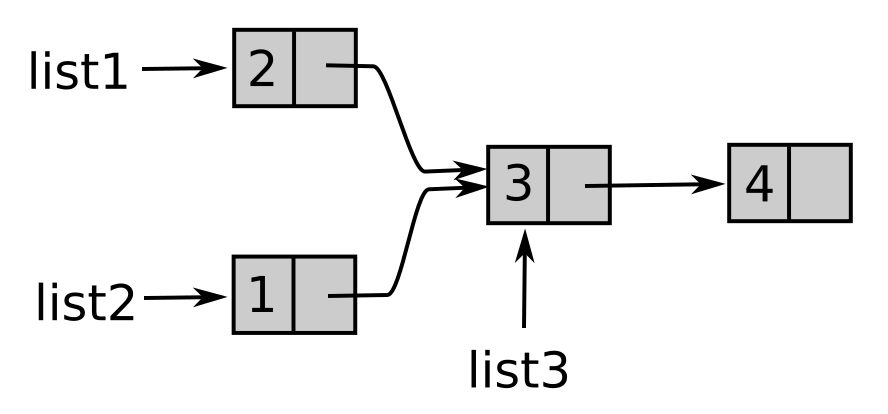
\includegraphics[width=0.5\textwidth]{lists.png}
\end{center}

Это позволяет сильно экономить память и делает операцию добавления в голову (cons) константной по трудоёмкости. Однако в конец списка добавить ничего нельзя, потому как если бы мы, например, добавили в конец list1 какой-то элемент, это добавление увидели бы list2 и list3, что нельзя, потому что списки немутабельны. Поэтому операция конкатенации копирует свой левый аргумент в новый список (а правый не копирует, кстати). Например, 

\begin{minted}{fsharp}
let list4 = list1 @ list3
\end{minted}

сделает нам новый список, у которого будут вначале копии элементов 2, 3 и 4, но элемент 4 будет ссылаться на элемент 3 из list3.

Почему списки немутабельны и как с этим жить --- это функциональный язык, тут изменяемое состояние не в почёте, и многие структуры данных реализованы так, чтобы их содержимое нельзя было менять. нет изменяемого состояния --- нет race condition-ов, нет неочевидных зависимостей по данным, можно легко менять порядок операций и т.д. и т.п. Если надо мутабельный список, всегда есть обычный дотнетовский System.Collections.Generic.List, но в первых домашках им пользоваться нельзя.

Ещё одна важная штука, отличающая F\# от более привычных, возможно, языков --- это то, что тут всякие интересные методы работы со списками вынесены в отдельный модуль. Это приём, используемый повсеместно в стандартной библиотеке --- есть какой-либо тип данных, который не умеет практически ничего и реально только хранит в себе данные, и есть отдельно класс, который модержит кучу статических методов, принимающих этот тип данных как параметр. Возможно, это кажется некрасивым с точки зрения ООП --- нарушается инкапсуляция --- но так у нас ФП. В F\# такой приём используется для того, чтобы помочь выводу типов (статический метод знает, какие типы аргументов он хочет, это сразу накладывает ограничения на используемые переменные) и для функций высших порядков, про которые чуть потом.

Со списками можно делать многое, но самое интересное в этой таблице: 
\begin{tabu} {| X[0.5 l p] | X[1 l p] | X[1 l p] | X[0.5 l p] |}
	\tabucline-
	Функция                & Описание                            & Пример                                              & Результат            \\
	\tabucline-
	\everyrow{\tabucline-}
	List.length            & Длина списка                        & $List.length\ [1;2;3]$                              & $3$                  \\
	List.nth               & n-ый элемент списка                 & $List.nth\ [1; 2; 3]\ 1$                            & $2$                  \\
	List.init              & Генерирует список                   & $List.init\ 3 (fun\ i\ \rightarrow\ i * i)$         & $[0; 1; 4]$          \\
	List.head              & Голова списка                       & $List.head\ [1; 2; 3]$                              & $1$                  \\
	List.tail              & Хвост списка                        & $List.tail\ [1; 2; 3]$                              & $[2; 3]$             \\
	List.map               & Применяет функцию ко всем элементам & $List.map\ (fun\ i\ \rightarrow\ i * i)\ [1; 2; 3]$ & $[1; 4; 9]$          \\
	List.filter            & Отбирает нужные элементы            & $List.filter\ (fun\ x\ \rightarrow\ x\ \%\ 2 <> 0)\ [1; 2; 3]$ & $[1; 3]$  \\
	List.fold              & "Свёртка"  & $List.fold\ (fun\ x\ acc\ \rightarrow\ acc * x)\ 1\ [1; 2; 3]$               & $6$                  \\
	List.zip               & Делает из двух списков список пар   & $List.zip\ [1; 2]\ [3; 4]$                          & $[(1, 3); (2, 4)]$   \\
\end{tabu}

Вообще, подробности в MSDN (\url{https://msdn.microsoft.com/visualfsharpdocs/conceptual/collections.list-module-\%5bfsharp\%5d}), старательно объяснять каждую функцию тут не будем, к тому же, они так или иначе знакомы по другим языкам (в C\# они называются немного по-другому, правда, но суть такая же).

Следующий важный тип, который потихоньку проникает в более традиционные языки --- это Option --- абстракция наличия либо отсутствия значения. Вот небольшой пример:

\begin{minted}{fsharp}
let people = [ ("Adam", None); ("Eve" , None);
    ("Cain", Some("Adam","Eve"));
    ("Abel", Some("Adam","Eve")) ]
\end{minted}

У Адама и Евы не было родителей, поэтому их родители обозначаются None, у Каина и Авеля родители были, поэтому они Some что-то. Вообще, Option это либо Some <какое-то значение>, либо None, поскольку Option генерик, то значение может быть любого типа (хоть список чего-нибудь ужасного). Вот пример использования:

\begin{minted}{fsharp}
let showParents (name, parents) =
    match parents with
    | Some(dad, mum) -> 
        printfn "%s, father %s, mother %s" name dad mum
    | None -> printfn "%s has no parents!" name
\end{minted}

\section{Функции}

Теперь немного подробнее про функции в F\#. Рекурсию мы уже видели:

\begin{minted}{fsharp}
let rec length l =
    match l with
    | [] -> 0
    | h :: t -> 1 + length t
\end{minted}

Но в F\# компилятор не допускает использования ещё не определённых имён (в отличие от C\#, где вполне можно вызывать метод, объявленный ниже), поэтому могут наступить проблемы с взаимной рекурсией. Собственно, взаимная рекурсия --- это плохо, она запутывает поток управления, но если очень надо, то взаимно рекурсивные функции надо описать рядом через ключевое слово and:

\begin{minted}{fsharp}
let rec even n = (n = 0u) || odd(n - 1u)
and odd n = (n <> 0u) && even(n - 1u)
\end{minted}

Обратите внимание на суффиксы \textit{u} у чисел --- это обозначение беззнакового целого литерала (просто 1 был бы знаковым int-ом).

Для функционального программирования очень важно такое соображение, что функция от n аргументов может быть представлена как функция от одного аргумента, возвращающая функцию от n - 1 аргумента --- это называется \textbf{каррирование}. Каррирование поддержано и синтаксически (кстати, поэтому в списке аргументов функций в F\# нет никаких скобок), и системой типов, что позволяет не передавать один из аргументов в функцию и получать функцию, которая хочет ещё аргументов. Зачем --- частичное применение, например:

\begin{minted}{fsharp}
let shift (dx, dy) (px, py) = (px + dx, py + dy)
let shiftRight = shift (1, 0)
let shiftUp = shift (0, 1)
let shiftLeft = shift (-1, 0)
let shiftDown = shift (0, -1)
\end{minted}

Можно это повызывать из F\# Interactive:

\begin{minted}{text}
> shiftDown (1, 1);;
val it : int * int = (1, 0)
\end{minted}

Практически полезно это не только тем, чтобы производить впечатление на коллег, но и для функций высших порядков. Например, как посчитать количество элементов сразу у пяти списков:

\begin{minted}{fsharp}
let lists = [[1; 2]; [1]; [1; 2; 3]; [1; 2]; [1]]
let lengths = List.map List.length lists
\end{minted}

List.length тут функция, принимающая один аргумент, который ей передаёт List.map, когда идёт по списку. Посмотрим, что будет, если функция над списком принимает два аргумента, например, тот же map. Положим, мы хотим возвести элементы всех пяти списков в квадрат:

\begin{minted}{fsharp}
let lists = [[1; 2]; [1]; [1; 2; 3]; [1; 2]; [1]]
let squares = List.map (List.map (fun x -> x * x)) lists
\end{minted}

Тут уже каррирование работает во всей красе, внутренний List.map возвращает функцию от одного аргумента типа ``список'', которую внешний List.map применяет к каждому элементу списка списков. Обратите внимание, что большинство функций из стандартной библиотеки принимают список последним аргументом, как раз для того, чтобы каррировать было удобнее.

Каррирование работает ещё лучше, если использовать оператор конвейера, или pipe forward:

\begin{minted}{fsharp}
let (|>) x f = f x
\end{minted}

Он просто принимает аргумент и функцию, и вызывает функцию, передавая ей аргумент. Зачем --- чтобы записывать вычисление в виде последовательно применяемых пребразований, вот так:

\begin{minted}{fsharp}
let sumFirst3 ls = ls |> Seq.take 3 |> Seq.fold (+) 0
\end{minted}

Согласитесь, это менее противоестественно, чем как бы жто выглядело на C\# или Java:

\begin{minted}{fsharp}
let sumFirst3 ls= Seq.fold (+) 0 (Seq.take 3 ls)
\end{minted}

Есть ещё оператор композиции, который почти как pipe forward, но позволяет аргумент функции в явном виде не писать:

\begin{minted}{fsharp}
let (>>) f g x = g (f x)

let sumFirst3 = Seq.take 3 >> Seq.fold (+) 0
let result = sumFirst3 [1; 2; 3; 4; 5]
\end{minted}

Его можно понимать как математическую композицию --- принимает две функции и возвращает функцию, которая сначала применяет первую функцию, затем вторую. А можно понимать как штуку, которая собирает конвейер, по которому потом пойдут данные. Сравните: 

\begin{minted}{fsharp}
let sumFirst3 = fun ls -> ls |> Seq.take 3 |> Seq.fold (+) 0
let sumFirst3 = Seq.take 3 >> Seq.fold (+) 0
\end{minted}

Есть ещё обратный конвейер и обратная композиция:

\begin{minted}{fsharp}
let (<|) f x = f x
let (<<) f g x = f (g x)
\end{minted}

Зачем, ведь обратный конвейер вообще ничего не делает? На самом деле, чтобы воспользоваться приоритетом операций и не ставить скобки там, где иначе пришлось бы их ставить:

\begin{minted}{fsharp}
printfn "Result = %d" <| factorial 5
\end{minted}

Сравните с

\begin{minted}{fsharp}
printfn "Result = %d" (factorial 5)
\end{minted}

\section{Использование библиотек .NET}

Как уже не раз говорилось, классы из .NET работают в F\# ``даром'', кроме того, F\# имеет ряд синтаксических особенностей, которые делают работу даже более приятной, чем ожидалось. Пример, небольшой текстовый редактор на Windows Forms, который грузит HTML-документ с удалённого адреса (правда, не умеет загружатьь отредактированный документ обратно):

\begin{minted}{fsharp}
open System.Windows.Forms

let form = new Form(Visible = false, TopMost = true, Text = "Welcome to F#")
let textB = new RichTextBox(Dock = DockStyle.Fill, Text = "Some text")
form.Controls.Add(textB)

open System.IO
open System.Net

/// Get the contents of the URL via a web request
let http (url: string) =
    let req = System.Net.WebRequest.Create(url)
    let resp = req.GetResponse()
    let stream = resp.GetResponseStream()
    let reader = new StreamReader(stream)
    let html = reader.ReadToEnd()
    resp.Close()
    html

textB.Text <- http("http://www.google.com")

form.ShowDialog() |> ignore
\end{minted}

\textit{open} --- это что-то вроде using, импорт имён из пространства имён. \textit{new Form} --- обычный вызов обычного конструктора, только в его параметры передаются не только параметры конструктора, но и значения public-свойств, которые мы хотим установить изначально. ``<-'' означает оператор присваивания (.NET-классы же мутабельны, их свойства можно менять, несмотря на то, что ссылка на объект не мутабельна). Функция ignore определена так:

\begin{minted}{fsharp}
let ignore x = ()
\end{minted}

Нужна она только для того, чтобы компилятор не выдввал предупреждение о неиспользованном значении, которое вернул метод \textit{form.ShowDialog}.

\section{Сопоставление шаблонов}

Тут уже несколько раз встречался оператор \textit{match}, настала пора рассказать про него поподробнее. Это почти как \textit{switch} в других языках, но немного круче, потому что позволяет тут же декомпозировать сложную структуру данных, сопоставляя переменную с шаблоном. Опять-таки, в C\# с версии 7.1 появилось что-то такое, но в силу ограниченности шаблонов в C\#, не такое выразительное, там можно матчить только по типу. В F\# же можно писать, например, так:

\begin{minted}{fsharp}
let urlFilter url agent =
    match (url, agent) with
    | "http://www.google.com", 99 -> true
    | "http://www.yandex.ru" , _ -> false
    | _, 86 -> true
    | _ -> false
\end{minted}

Подчёркивание означает ``что угодно'', и обратите внимание на два последних случая, в первом из них подчёркивание относится к первому элементу пары, во втором --- ко всей паре сразу.

Или вот так (пример с одного из предыдущих слайдов):

\begin{minted}{fsharp}
let rec length l =
    match l with
    | [] -> 0
    | h :: t -> 1 + length t
\end{minted}

Тут мы смотрим, если список пустой, то его длина 0, если нет, то в нём есть голова - cons - хвост, и его длина --- это длина его хвоста плюс 1.

Есть ещё ключевое слово when, позволяющее указать в match произвольное булевое условие:

\begin{minted}{fsharp}
let sign x =
    match x with
    | _ when x < 0 -> -1
    | _ when x > 0 -> 1
    | _ -> 0
\end{minted}

Это довольно странно делать match-ем, но в каком-то смысле получилось красивее, чем последовательность if-ов.

Однако важно понимать, что F\# не пытается в match считать переменные с одинаковыми именами одной переменной (как делает, например, Prolog), потому что это привело бы к резкому увеличению трудоёмкости match-а (до экспоненциальной, как в Prolog). Например, вот так работать не будет:

\begin{minted}{fsharp}
let isSame pair =
    match pair with
    | (a, a) -> true
    | _ -> false
\end{minted}

А вот так будет:

\begin{minted}{fsharp}
let isSame pair =
    match pair with
    | (a, b) when a = b -> true
    | _ -> false
\end{minted}

Какие шаблоны ещё можно использовать в match (и, кстати, в let):

\begin{tabu} {| X[0.9 l p] | X[1 l p] | X[1 l p] |}
	\tabucline-
	Синтаксис                               & Описание                  & Пример                  \\
	\tabucline-
	\everyrow{\tabucline-}
	$(pat, \ldots, pat)$                    & Кортеж                    & $(1, 2, (``3``, x))$    \\
	$[pat; \ldots; pat]$                    & Список                    & $[x; y; 3]$             \\
	$pat :: pat$                            & cons                      & $h :: t$                \\
	$pat\ |\ pat$                           & "Или"                     & $[x]\ |\ [``X``\ |\ x]$ \\
	$pat\ \&\ pat$                          & "И"                       & $[p] \& [(x, y)]$       \\
	$pat\ as\ id$                           & Именованный шаблон        & $[x]\ as\ inp$          \\
	$id$                                    & Переменная                & $x$                     \\
	$\_$                                    & Wildcard (что угодно)     & $\_$                    \\
	литерал                                 & Константа                 & $239, DayOfWeek.Monday$ \\
	$:?\ type$                              & Проверка на тип           & $:?\ string$            \\
\end{tabu}

\section{Юнит-тестирование в F\#}

Теперь про юнит-тестирование, штуку, хоть и не связанную с функциональным программированием напрямую, но имеющую в F\# несколько приятных функциональных особенностей. Кстати, теперь юнит-тесты в домашке обязательны.

Поскольку F\# компилируется в байт-коды .NET, то нет никаких причин не работать стандартным библиотекам модульного тестирования, которые работают и в C\#, например, NUnit, Microsoft Testing Framework и т.д. Ими вполне можно пользоваться, но есть более красивые с функциональной точки зрения обёртки над ними, которые позволят писать тесты в более F\#-овом стиле, прежде всего FsUnit, стандарт де-факто в модульном тестировании для F\#. Есть и библиотеки, специфичные для F\#: FsCheck и Unquote, например (на самом деле, не совсем для F\#, FsCheck портирована с Хаскеля, но в C\# точно нет ничего такого --- хотя никто не мешает тесты для программ на C\# писать на F\#-е, естественно, пользуясь его тулами).

Вот небольшой пример теста с FsUnit-ом:

\begin{minted}{fsharp}
module ``Project Euler - Problem 1`` =
    open NUnit.Framework
    open FsUnit

    let GetSumOfMultiplesOf3And5 max =
        seq{3 .. max - 1} 
        |> Seq.fold(fun acc number ->
                    (if (number % 3 = 0 || number % 5 = 0) then
                         acc + number else acc)) 0

    [<Test>]
    let ``Sum of multiples of 3 and 5 to 10 should return 23`` () =
        GetSumOfMultiplesOf3And5(10) |> should equal 23
\end{minted}

Тут показан, кстати, способ записи идентификаторов через двойные апострофы --- вся строка внутри считается именем, даже если там пробелы, ключевые слова и прочая жесть. Сам тест помечен атрибутом \textit{[<Test>]}, и вообще в F\# атрибуты пишутся в скобках вида [< >] (потому что просто квадратные скобки, как в C\#, заняты под списки). \textit{should equal} --- это что-то вроде \textit{Assert.Equals}, только круче.

Круче тем, что условие, которое надо проверить, на самом деле может быть довольно сложным, не просто равенство-истинность-не null, как принято в C\#. Условие записывается в виде так называемых \textit{матчеров}. Для тех, кто в курсе, такой же подход используется в библиотеке Hamcrest/NHamcrest. Вот примеры, из которых по идее всё должно стать понятно:

\begin{minted}{fsharp}
1 |> should equal 1
1 |> should not' (equal 2)
10.1 |> should (equalWithin 0.1) 10.11
"ships" |> should startWith "sh"
"ships" |> should not' (endWith "ss")
"ships" |> should haveSubstring "hip"
[1] |> should contain 1
[] |> should not' (contain 1)
anArray |> should haveLength 4

(fun () -> failwith "BOOM!" |> ignore) 
    |> should throw typeof<System.Exception>

shouldFail (fun () -> 5/0 |> ignore)
\end{minted}

Есть некоторые заморочки с should throw и shouldFail, они хотят функцию без аргументов, возвращающую ничего, поэтому при вызове настоящий код обёрнут в лямбду.

Вот ещё примеры матчеров:

\begin{minted}{fsharp}
true |> should be True
false |> should not' (be True)
"" |> should be EmptyString
null |> should be Null

anObj |> should not' (be sameAs otherObj)

11 |> should be (greaterThan 10)
10.0 |> should be (lessThanOrEqualTo 10.1)

0.0 |> should be ofExactType<float>
1 |> should not' (be ofExactType<obj>)

Choice<int, string>.Choice1Of2(42) |> should be (choice 1)

"test" |> should be instanceOfType<string>
"test" |> should not' (be instanceOfType<int>)

2.0 |> should not' (be NaN)

[1; 2; 3] |> should be unique

[1; 2; 3] |> should be ascending
[1; 3; 2] |> should not' (be ascending)
[3; 2; 1] |> should be descending
[3; 1; 2] |> should not' (be descending)
\end{minted}

Более интересная, хотя и реже используемая штука --- это FsCheck. FsCheck берёт функцию, рефлексией понимает, что функция принимает, и генерирует случайные значения её параметрам, после чего сколько-то раз её вызывает. Функция должна возвращать булевое значение. Если функция вернёт false, то FsCheck скажет, что тест провален, и ещё и покажет минимальный контрпример, на котором, собственно, получилось плохо. Например: 

\begin{minted}{fsharp}
open FsCheck

let revRevIsOrig (xs:list<int>) = List.rev(List.rev xs) = xs

Check.Quick revRevIsOrig
// Ok, passed 100 tests.

let revIsOrig (xs:list<int>) = List.rev xs = xs
Check.Quick revIsOrig
// Falsifiable, after 2 tests (2 shrinks) (StdGen (338235241,296278002)):
// Original:
// [3; 0]
// Shrunk:
// [1; 0]
\end{minted}

Замечу, что FsCheck прекрасно работает в паре с FsUnit (бросает исключение, которое FsUnit ловит и помечает тест как проваленный), так что писать часть тестов руками, а часть отдавать FsCheck не зазорно и повышает качество кода.

Ещё одна интересная библиотека --- это Unquote. Вообще, она просто интерпретатор F\#-а, использующий встроенный в язык механизм Quotation-ов, дающий возможность в программе получить дерево разбора куска кода на F\#, потом обходить его как обычное дерево и делать с ним что угодно. Unquote хороша тем, что умеет не просто сказать, прошёл тест или нет, но и если не прошёл, показать последовательность преобразований, которая привела к ошибке. Вот пример:

\begin{minted}{fsharp}
[<Test>]
let ``Unquote demo`` () =
    test <@ ([3; 2; 1; 0] |> List.map ((+) 1)) = [1 + 3..1 + 0] @>

// ([3; 2; 1; 0] |> List.map ((+) 1)) = [1 + 3..1 + 0]
// [4; 3; 2; 1] = [4..1]
// [4; 3; 2; 1] = []
// false
\end{minted}

Эти ``<@'' и ``@>'' и есть границы quotation-а, всё, что внутри, не вычисляется, а превращается в дерево разбора, которое отдаётся функции test из Unquote.

И конечно, библиотека для создания mock-объектов. В случае F\#-а это Foq, тоже использующая quotation-ы, но на сей раз для генерации моков. Вот пример:

\begin{minted}{fsharp}
[<Test>]
let ``Foq demo`` () =
    let mock = Mock<System.Collections.Generic.IList<int>>()
                .Setup(fun x -> <@ x.Contains(any()) @>).Returns(true)
                .Create()

    mock.Contains 1 |> Assert.True
\end{minted}

Этот мок имитирует мутабельный список, который на запрос Contains всегда возвращает true. Собственно, тоже хорошо работает с FsUnit и NUnit, можно использовать, чтобы красиво генерить тестовые заглушки и уменьшать зависимость теста от других кусков программы.

\end{document}
